\documentclass[tikz,border=0pt]{standalone}
\usepackage[T1]{fontenc}
\usetikzlibrary{arrows.meta,shapes.geometric}
\usepackage[sfdefault,lining]{FiraSans}
\definecolor{ink}{HTML}{23373B}
\definecolor{accent}{HTML}{EB811B}
\definecolor{primary}{HTML}{9FCFCC}
\definecolor{store}{HTML}{D3DADD}
\definecolor{zone}{HTML}{F2F5F6}
\newcommand{\ev}[1]{{\textbf{E}\;\texttt{#1}}}
\tikzset{
 every node/.style={font=\sffamily\fontsize{9}{11}\selectfont,text=ink},
 box/.style={draw=none,fill=primary,align=center,inner sep=2mm,text width=42mm},
 state/.style={box,rounded corners=2mm},
 bad/.style={state,fill=white,draw=accent,line width=.8pt},
 guard/.style={diamond,aspect=3,draw=ink,fill=white,line width=.65pt,align=center,inner sep=.8mm,text width=38mm},
 external/.style={box,dashed,fill=white,draw=ink,line width=.6pt},
 flow/.style={-{Stealth[length=2mm]},draw=ink,line width=.7pt},
 reject/.style={flow,draw=accent,densely dashed},
 port/.style={circle,draw=none,fill=ink,text=white,inner sep=0pt,minimum size=5mm,font=\sffamily\bfseries\fontsize{9}{11}\selectfont},
 note/.style={align=left,anchor=west,inner sep=0pt},
 heading/.style={anchor=west,font=\sffamily\bfseries\fontsize{10}{12}\selectfont},
 tag/.style={fill=zone,inner sep=1pt},
 panel/.style={draw=none,fill=zone,rounded corners=3pt}
}
\begin{document}
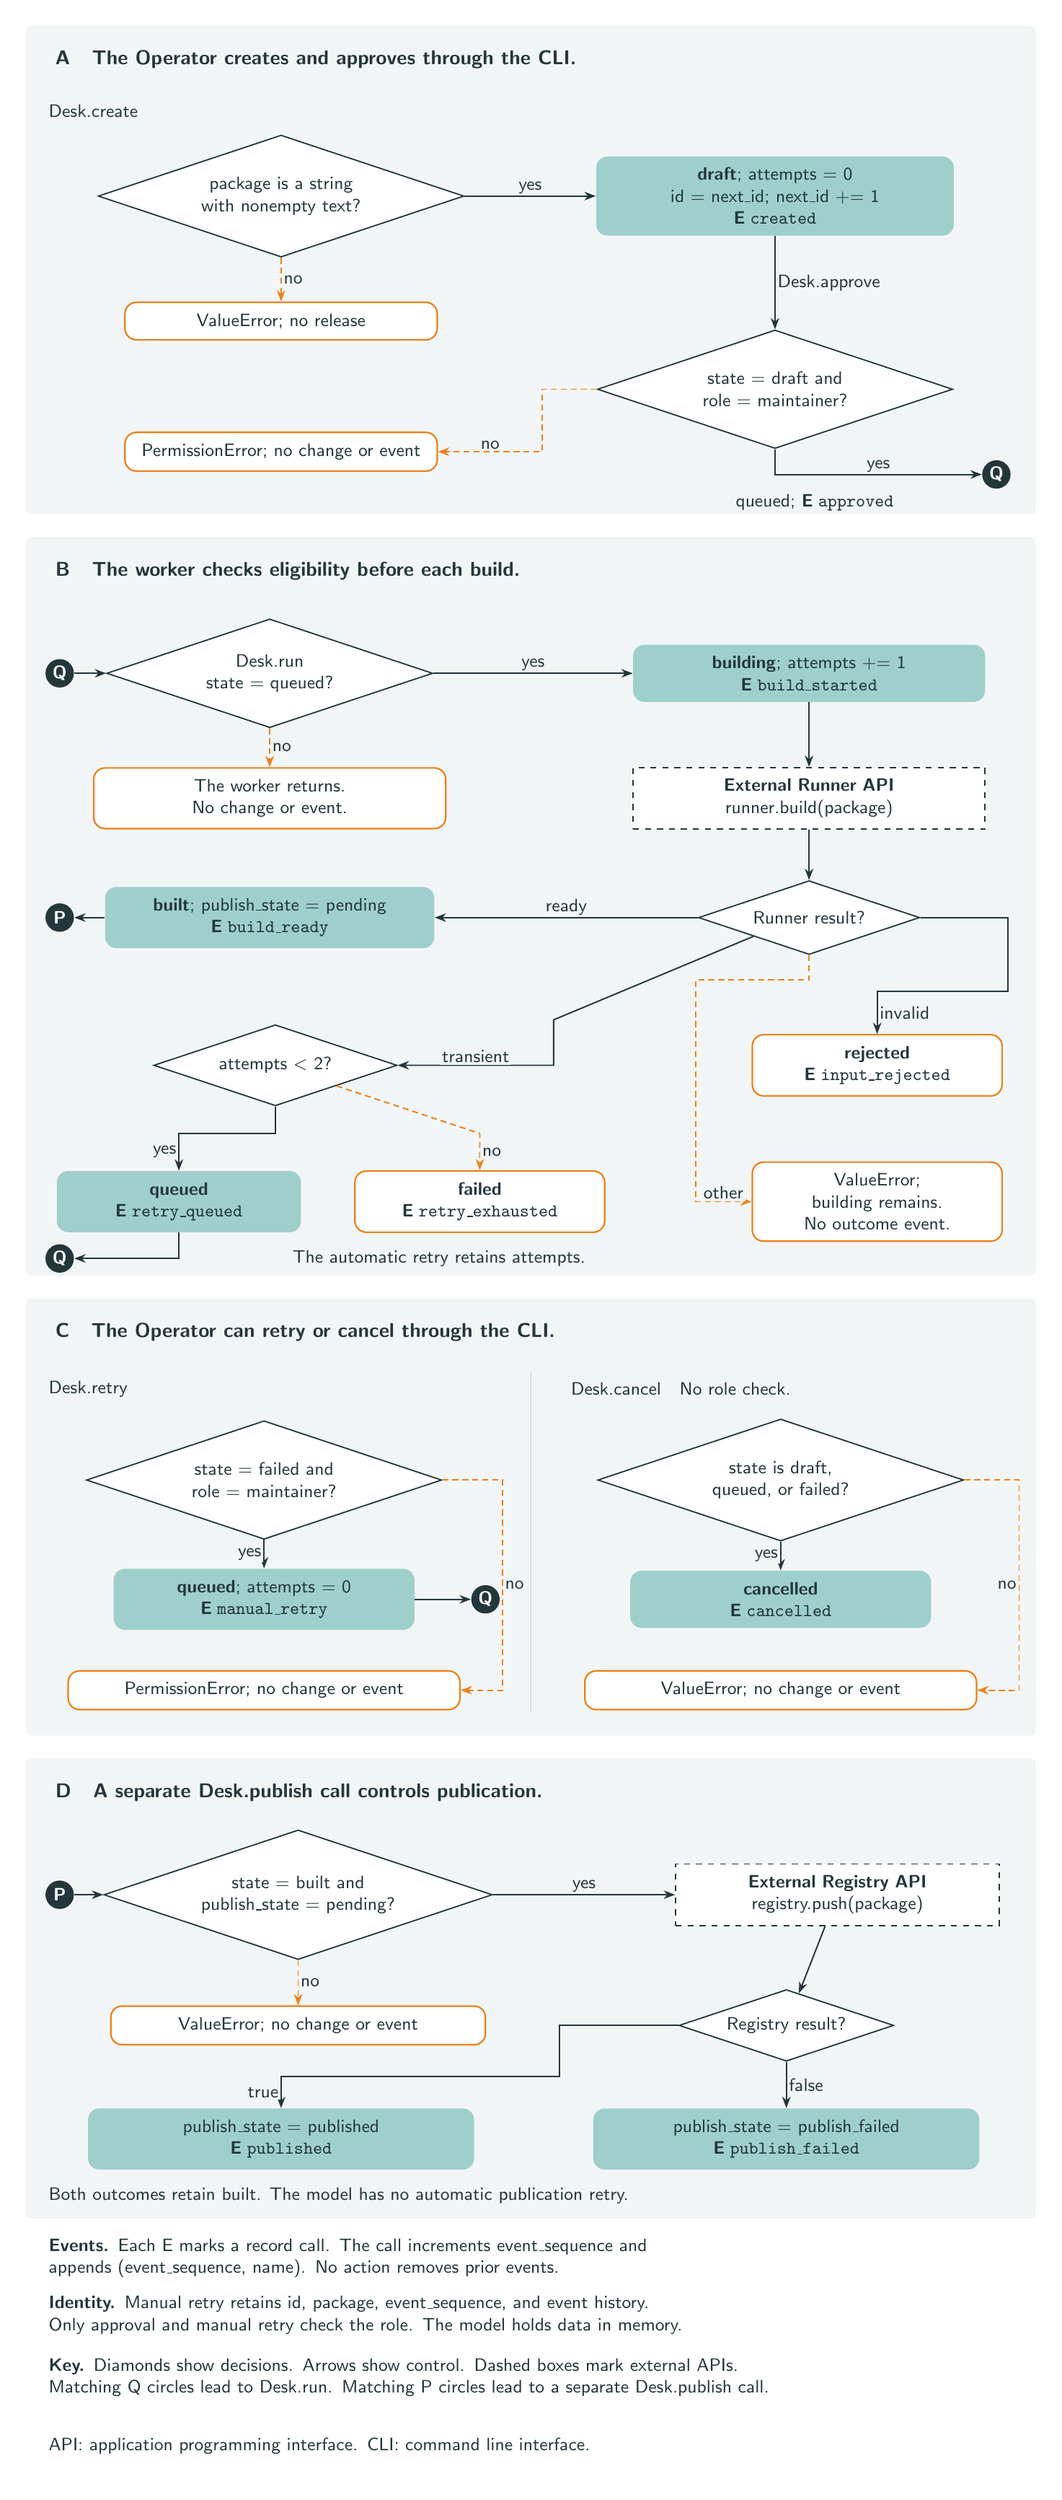
\begin{tikzpicture}[x=1mm,y=-1mm]
\path[use as bounding box] (0,0) rectangle (180,433);
\draw[panel] (1,1) rectangle (179,87);
\node[heading] at (5,7) {A\quad The Operator creates and approves through the CLI.};
\node[note] at (5,16) {Desk.create};
\node[guard] (input) at (46,31) {package is a string\\with nonempty text?};
\node[state,text width=59mm] (draft) at (133,31) {\textbf{draft}; attempts = 0\\id = next\_id; next\_id += 1\\\ev{created}};
\draw[flow] (input) -- node[tag,above] {yes} (draft);
\node[bad,text width=51mm] (inputbad) at (46,53) {ValueError; no release};
\draw[reject] (input) -- node[tag,right] {no} (inputbad);
\node[guard] (approve) at (133,65) {state = draft and\\role = maintainer?};
\draw[flow] (draft) -- node[tag,right] {Desk.approve} (approve);
\node[bad,text width=51mm] (denied) at (46,76) {PermissionError; no change or event};
\draw[reject] (approve.west) -- (92,65) -- (92,76) -- node[tag,above] {no} (denied);
\node[port] (qa) at (172,80) {Q};
\draw[flow] (approve.south) -- (133,80) -- node[tag,above] {yes} (qa);
\node[tag] at (140,85) {queued; \ev{approved}};

\draw[panel] (1,91) rectangle (179,221);
\node[heading] at (5,97) {B\quad The worker checks eligibility before each build.};
\node[port] (qb) at (7,115) {Q};
\node[guard,text width=31mm] (eligible) at (44,115) {Desk.run\\state = queued?};
\draw[flow] (qb) -- (eligible);
\node[state,text width=58mm] (start) at (139,115) {\textbf{building}; attempts += 1\\\ev{build\_started}};
\draw[flow] (eligible) -- node[tag,above] {yes} (start);
\node[bad,text width=58mm] (skip) at (44,137) {The worker returns.\\No change or event.};
\draw[reject] (eligible) -- node[tag,right] {no} (skip);
\node[external,text width=58mm] (runner) at (139,137) {\textbf{External Runner API}\\runner.build(package)};
\draw[flow] (start) -- (runner);
\node[guard,text width=26mm] (outcome) at (139,158) {Runner result?};
\draw[flow] (runner) -- (outcome);
\node[state,text width=54mm] (ready) at (44,158) {\textbf{built}; publish\_state = pending\\\ev{build\_ready}};
\draw[flow] (outcome) -- node[tag,above] {ready} (ready);
\node[port] (pb) at (7,158) {P};
\draw[flow] (ready) -- (pb);
\node[bad,text width=40mm] (invalid) at (151,184) {\textbf{rejected}\\\ev{input\_rejected}};
\draw[flow] (outcome.east) -- (174,158) -- (174,171) -- (151,171) -- node[tag,right] {invalid} (invalid);
\node[bad,text width=40mm] (unknown) at (151,208) {ValueError;\\building remains.\\No outcome event.};
\draw[reject] (outcome.south) -- (139,169) -- (119,169) -- (119,208) -- node[tag,above] {other} (unknown);
\node[guard,text width=28mm] (limit) at (45,184) {attempts $<$ 2?};
\draw[flow] (outcome.south west) -- (94,176) -- (94,184) -- node[tag,above] {transient} (limit);
\node[state,text width=39mm] (again) at (28,208) {\textbf{queued}\\\ev{retry\_queued}};
\node[bad,text width=40mm] (failed) at (81,208) {\textbf{failed}\\\ev{retry\_exhausted}};
\draw[flow] (limit.south) -- (45,196) -- (28,196) -- node[tag,left] {yes} (again);
\draw[reject] (limit.south east) -- (81,196) -- node[tag,right] {no} (failed);
\node[port] (qr) at (7,218) {Q};
\draw[flow] (again.south) -- (28,218) -- (qr);
\node[note] at (48,218) {The automatic retry retains attempts.};

\draw[panel] (1,225) rectangle (179,302);
\node[heading] at (5,231) {C\quad The Operator can retry or cancel through the CLI.};
\draw[draw=ink!25] (90,238) -- (90,298);
\node[note] at (5,241) {Desk.retry};
\node[note] at (97,241) {Desk.cancel\quad No role check.};
\node[guard] (retry) at (43,257) {state = failed and\\role = maintainer?};
\node[guard] (cancel) at (134,257) {state is draft,\\queued, or failed?};
\node[state,text width=49mm] (reset) at (43,278) {\textbf{queued}; attempts = 0\\\ev{manual\_retry}};
\node[state,text width=49mm] (cancelled) at (134,278) {\textbf{cancelled}\\\ev{cancelled}};
\draw[flow] (retry.south) -- node[tag,left] {yes} (reset.north);
\draw[flow] (cancel.south) -- node[tag,left] {yes} (cancelled.north);
\node[port] (qc) at (82,278) {Q};
\draw[flow] (reset) -- (qc);
\node[bad,text width=65mm] (retrybad) at (43,294) {PermissionError; no change or event};
\node[bad,text width=65mm] (cancelbad) at (134,294) {ValueError; no change or event};
\draw[reject] (retry.east) -- (85,257) -- node[tag,right] {no} (85,294) -- (retrybad);
\draw[reject] (cancel.east) -- (176,257) -- node[tag,left] {no} (176,294) -- (cancelbad);

\draw[panel] (1,306) rectangle (179,387);
\node[heading] at (5,312) {D\quad A separate Desk.publish call controls publication.};
\node[port] (pd) at (7,330) {P};
\node[guard,text width=42mm] (publish) at (49,330) {state = built and\\publish\_state = pending?};
\draw[flow] (pd) -- (publish);
\node[external,text width=53mm] (registry) at (144,330) {\textbf{External Registry API}\\registry.push(package)};
\draw[flow] (publish) -- node[tag,above] {yes} (registry);
\node[bad,text width=62mm] (pubbad) at (49,353) {ValueError; no change or event};
\draw[reject] (publish) -- node[tag,right] {no} (pubbad);
\node[guard,text width=23mm] (result) at (135,353) {Registry result?};
\draw[flow] (registry) -- (result);
\node[state,text width=64mm] (published) at (46,373) {publish\_state = published\\\ev{published}};
\node[state,text width=64mm] (pubfail) at (135,373) {publish\_state = publish\_failed\\\ev{publish\_failed}};
\draw[flow] (result.west) -- (95,353) -- (95,362) -- (46,362) -- node[tag,left] {true} (published);
\draw[flow] (result.south) -- node[tag,right] {false} (pubfail.north);
\node[note] at (5,383) {Both outcomes retain built. The model has no automatic publication retry.};

\node[note,text width=170mm] at (5,394) {\textbf{Events.} Each E marks a record call. The call increments event\_sequence and\\appends (event\_sequence, name). No action removes prior events.};
\node[note,text width=170mm] at (5,404) {\textbf{Identity.} Manual retry retains id, package, event\_sequence, and event history.\\Only approval and manual retry check the role. The model holds data in memory.};
\node[note,text width=170mm] at (5,415) {\textbf{Key.} Diamonds show decisions. Arrows show control. Dashed boxes mark external APIs.\\Matching Q circles lead to Desk.run. Matching P circles lead to a separate Desk.publish call.};
\node[note,text width=170mm] at (5,427) {API: application programming interface. CLI: command line interface.};
\end{tikzpicture}
\end{document}
